\chapter{Planification}

\section{Methodology}
In the degree, we usually use a waterfall model (see figure \ref{fig:planification_waterfall_model}) to develop software. For small projects and use cases this methodology
works fine, but in bigger projects it carries a lot of issues (late detection of errors related to analysis and design, testing late and difficulty to change or add new requisites).
In addition, due to my limited experience I think an agile methodology would fit to a development
process that overlaps with learning phases. \\

\begin{figure}[H]
    \begin{center}
        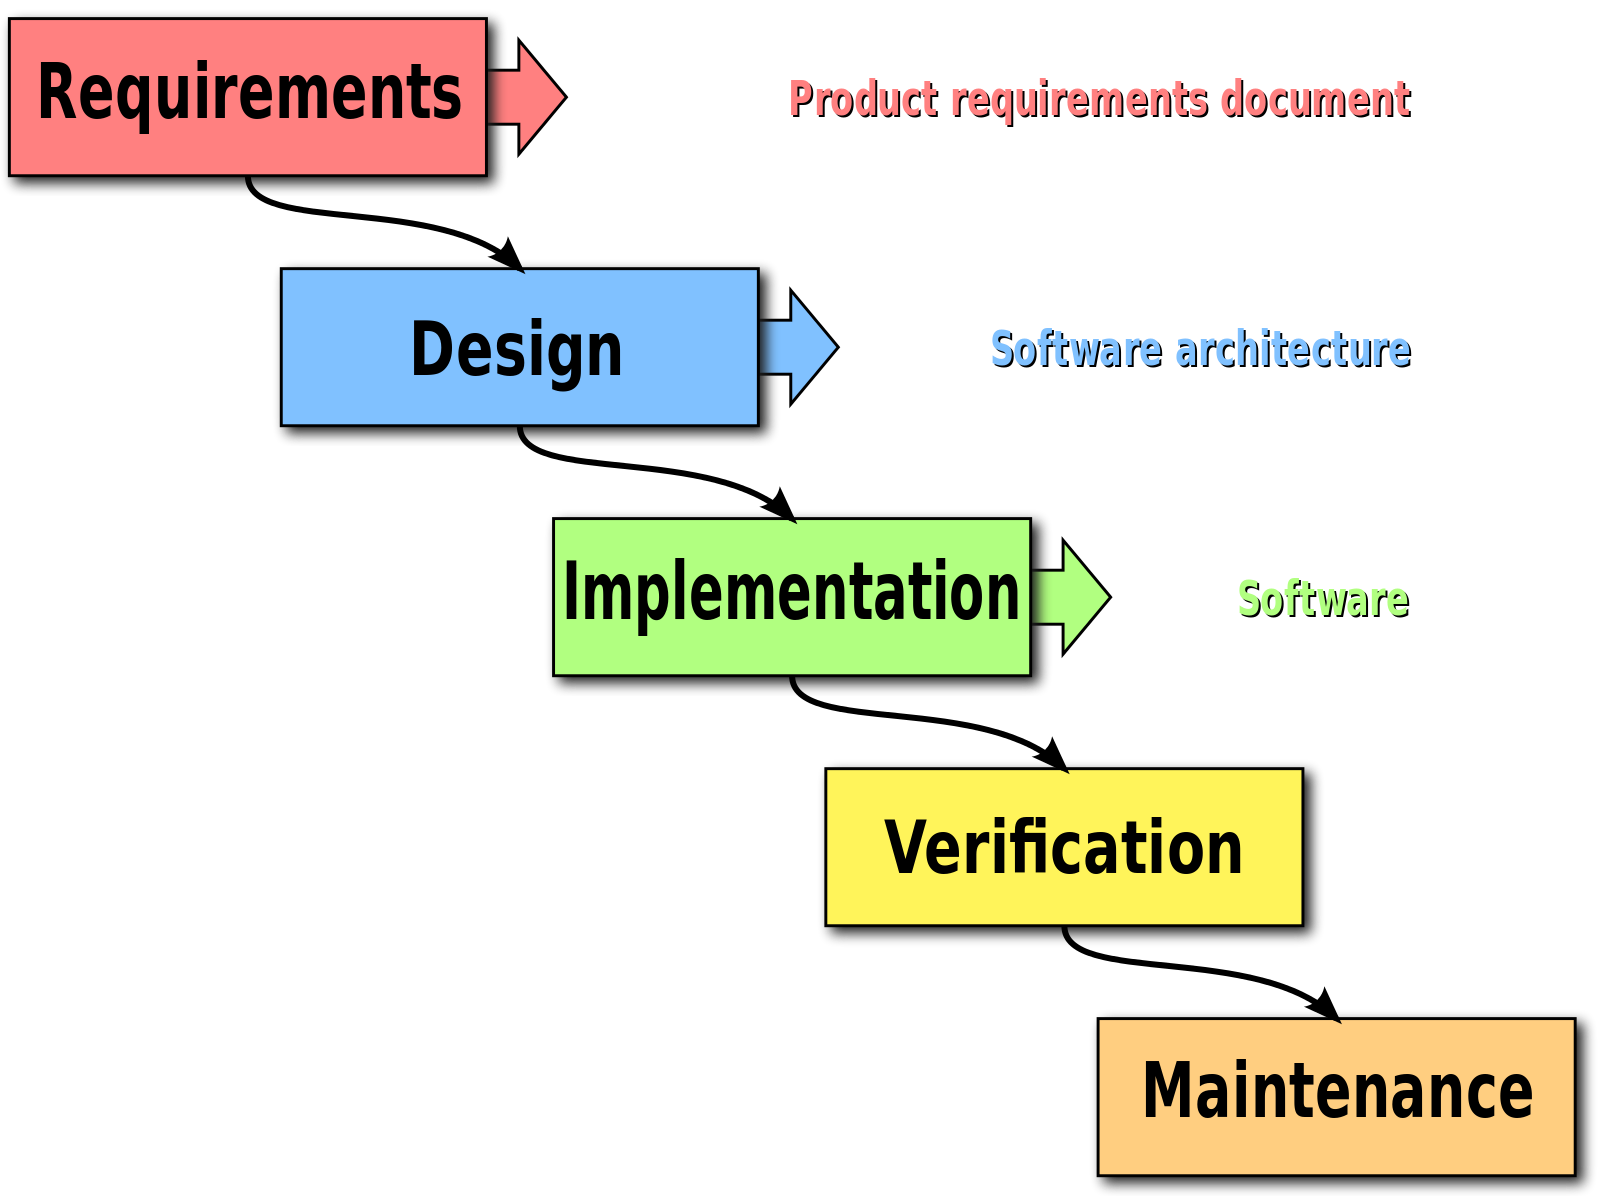
\includegraphics[width=0.4\textwidth]{assets/waterfall_model.png}
        \caption{Waterfall Model. \cite{Waterfall}}
        \label{fig:planification_waterfall_model}
    \end{center}
\end{figure}

Although the Scrum model (see figure \ref{fig:planification_scrum_model}) uses fixed time sprints, I decided to use sprints of variable duration as 
the time that could be devoted to the project was not constant. Each sprint was designed in terms of 
the value added.

\begin{figure}[H]
    \begin{center}
        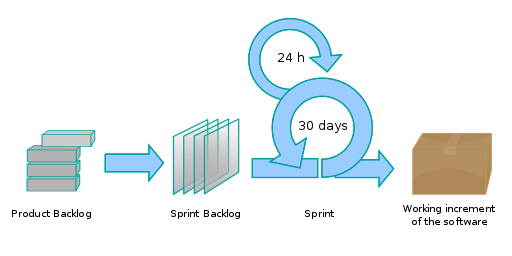
\includegraphics[width=0.4\textwidth]{assets/scrum.png}
        \caption{Scrum Model. \cite{Scrum}}
        \label{fig:planification_scrum_model}
    \end{center}
\end{figure}

Firstly, I identified all the tasks that I would have to complete to develop the application and the thesis itself. These tasks are:
\begin{itemize}[noitemsep]
    \item Literature review
    \item Backend
    \item Frontend
    \item Deep Learning service
    \item Documentation
    \item Design
\end{itemize}

Each sprint contained subtasks of the previous list and where associated with a milestone.
Each milestone added value with respect to the previous one and was validated by my advisor.

\section{Project schedule}

In order to create my project schedule, I used Notion \cite{Notion}. Notion's schedule information can be checked \href{https://cyclic-chiller-238.notion.site/LearnASL-60bb8f91ed8f4ccfa90f98ee2306403d}{here}. \\

\subsection{Initial project schedule (v0)}
\begin{table}[H]
    \centering
    \resizebox{\textwidth}{!}{
    \begin{tabular}{|l|l|l|l|}
        \cline{1-4}      Name                                &    Milestone                                                              &    Due                                           &       State   \\
        \hline           Project set up                      &    \href{https://github.com/JesusGonzalezA/LearnASL/milestone/1}{Link}      &    November 12, 2021                             &       No      \\
        \hline           Graphical Stats                     &    \href{https://github.com/JesusGonzalezA/LearnASL/milestone/8}{Link}      &    February 4, 2022    →   February 11, 2022     &       No      \\
        \hline           The app saves info                  &    \href{https://github.com/JesusGonzalezA/LearnASL/milestone/7}{Link}      &    January 7, 2022     →   January 14, 2022      &       No      \\
        \hline           The app can create tests            &    \href{https://github.com/JesusGonzalezA/LearnASL/milestone/4}{Link}      &    December 31, 2021   →   January 7, 2022       &       No      \\
        \hline           Frontend avalaible                  &    \href{https://github.com/JesusGonzalezA/LearnASL/milestone/3}{Link}      &    December 10, 2021   →   December 31, 2021     &       No      \\
        \hline           The app is designed                 &    \href{https://github.com/JesusGonzalezA/LearnASL/milestone/2}{Link}      &    December 3, 2021    →   December 17, 2021     &       No      \\
        \hline           The user is authenticated           &    \href{https://github.com/JesusGonzalezA/LearnASL/milestone/6}{Link}      &    November 12, 2021   →   December 3, 2021      &       No      \\
        \hline           The app validates the videos        &    \href{https://github.com/JesusGonzalezA/LearnASL/milestone/5}{Link}      &    February 11, 2022   →   February 25, 2022     &       No      \\
        \hline           Using own ML model                  &    \href{https://github.com/JesusGonzalezA/LearnASL/milestone/10}{Link}     &                                                  &       No      \\
        \hline           Migrating to React Native or PWA    &    \href{https://github.com/JesusGonzalezA/LearnASL/milestone/9}{Link}      &                                                  &       No      \\
        \hline
    \end{tabular}
    }
\caption{Initial project schedule - v0}
\label{table:planification_theorical_project_schedule}
\end{table}

\subsection{Re-scheduling the project}
I changed the order of the milestones (see table \ref{table:planification_real_v1}). I decided to develop the backend of the application first, instead of the frontend or implementing them in the same time. \\

This decision was made because focusing on the same technology would allow me to go faster because I was learning ASP.NET core in my
university, so I could ask my teachers for help and it also helped me to study. \\
\begin{table}[H]
    \centering
    \resizebox{\textwidth}{!}{
    \begin{tabular}{|l|l|l|l|l|}
        \cline{1-5}      Name                                           &    Milestone                                              &       Due                                     & State & Tag       \\
        \hline           Project set up                                 & \href{https://github.com/JesusGonzalezA/LearnASL/milestone/1}{Link}    &       November 12, 2021                       & Yes   & Backend, Frontend \\
        \hline           Implement authorization and authentication     & \href{https://github.com/JesusGonzalezA/LearnASL/milestone/6}{Link}    &       November 12, 2021 → December 3, 2021    & Yes   & Backend   \\
        \hline           The app can create tests: just word to video   &                                                        &       December 3, 2021  → January 7, 2022      & No    & Backend   \\
        \hline           The app can create the rest of tests           & \href{https://github.com/JesusGonzalezA/LearnASL/milestone/4}{Link}    &       January 7, 2022   → January 21, 2022      & No    & Backend   \\
        \hline           The app create stats                           & \href{https://github.com/JesusGonzalezA/LearnASL/milestone/8}{Link}    &       January 21, 2022  → January 28, 2022     & No    & Backend   \\
        \hline           The app is designed                            & \href{https://github.com/JesusGonzalezA/LearnASL/milestone/2}{Link}    &       January 28, 2022  → February 4, 2022     & No    & Frontend  \\
        \hline           Frontend avalaible                             & \href{https://github.com/JesusGonzalezA/LearnASL/milestone/3}{Link}    &       February 4, 2022  → March 4, 2022        & No    & Frontend  \\
        \hline           Connect frontend and backend                   &                                                         &       March 4, 2022     → March 11, 2022          & No    & Frontend  \\
        \hline           The app validates the videos                   & \href{https://github.com/JesusGonzalezA/LearnASL/milestone/5}{Link}    &       March 11, 2022    → April 1, 2022          & No    & Backend   \\
        \hline           Using own ML model                             & \href{https://github.com/JesusGonzalezA/LearnASL/milestone/10}{Link}   &                                               & No    & Backend   \\
        \hline           Migrating to React Native or PWA               & \href{https://github.com/JesusGonzalezA/LearnASL/milestone/9}{Link}    &                                               & No    & Frontend  \\
        \hline
    \end{tabular}
    }
\caption{Project schedule - v1}
\label{table:planification_real_v1}
\end{table}

The next modification (see table \ref{table:planification_real_v2}) was made because I did not take into account the task of documenting what I was implementing, and I had to subdivide the \textit{Frontend} task as well. \\

Also, I underestimated the time required to do unit tests as I had to learn about additional aspects by myself. \\
\begin{table}[H]
    \centering
    \resizebox{\textwidth}{!}{
    \begin{tabular}{|l|l|l|l|l|}
        \cline{1-5}      Name                                           &    Milestone                                              &       Due   & State & Tag  \\
        \hline Project set up & \href{https://github.com/JesusGonzalezA/LearnASL/milestone/1}{Link} & November 12, 2021 & Yes & Backend, Frontend    \\
        \hline Implement authorization and authentication & \href{https://github.com/JesusGonzalezA/LearnASL/milestone/6}{Link} & November 12, 2021 → December 3, 2021 & Yes & Backend   \\
        \hline The app can create tests & \href{https://github.com/JesusGonzalezA/LearnASL/milestone/4}{Link} & December 3, 2021 → January 7, 2022 & Yes & Backend   \\
        \hline The app create stats & \href{https://github.com/JesusGonzalezA/LearnASL/milestone/8}{Link} & January 1, 202 → January 7, 202 & Yes & Backend  \\
        \hline Documentate &  & January 6, 2022 → January 11, 2022 & Yes & Backend  \\
        \hline Integration tests API &  & January 12, 2022 → January 26, 2022 & No & Backend    \\
        \hline The app is designed & \href{https://github.com/JesusGonzalezA/LearnASL/milestone/2}{Link} & January 26, 2022 → February 4, 2022 & No & Frontend   \\
        \hline User management &  & February 4, 2022 → February 11, 2022 & No & Frontend    \\
        \hline Test management &  & February 11, 2022 → February 21, 2022 & No & Frontend   \\
        \hline Stats management &  & February 21, 2022 → February 28, 2022 & No & Frontend  \\
        \hline The app validates the videos & \href{https://github.com/JesusGonzalezA/LearnASL/milestone/5}{Link} & February 28, 2022 → March 20, 2022 & No & Backend    \\
        \hline Using own ML model & \href{https://github.com/JesusGonzalezA/LearnASL/milestone/10}{Link} &  & No & Backend   \\
        \hline Migrating to React Native or PWA & \href{https://github.com/JesusGonzalezA/LearnASL/milestone/9}{Link} &  & No & Frontend \\
        \hline Integrate with google analytics &  &  & No & Frontend \\
        \hline
    \end{tabular}
    }
\caption{Project schedule - v2}
\label{table:planification_real_v2}
\end{table}

The next modification (see table \ref{table:planification_real_v3}) was made because I overestimed the time required to learn the unit testing framework. This 
allowed me to have some extra days devoted to rest and design the application. \\
\begin{table}[H]
    \centering
    \resizebox{\textwidth}{!}{
    \begin{tabular}{|l|l|l|l|l|}
        \cline{1-5}      Name                                           &    Milestone                                              &       Due   & State & Tag  \\
        \hline Project set up & \href{https://github.com/JesusGonzalezA/LearnASL/milestone/1}{Link} & November 12 , 2021 & Yes & Backend, Frontend \\
        \hline Implement authorization and authentication & \href{https://github.com/JesusGonzalezA/LearnASL/milestone/6}{Link} & November 12 , 2021 → December 3 , 2021 & Yes & Backend \\
        \hline The app can create tests & \href{https://github.com/JesusGonzalezA/LearnASL/milestone/4}{Link} & December 3 , 2021 → January 7 , 2022 & Yes & Backend \\
        \hline The app create stats & \href{https://github.com/JesusGonzalezA/LearnASL/milestone/8}{Link} & January 1 , 202 → January 7 , 202 & Yes & Backend \\
        \hline Documentate &  & January 6 , 2022 → January 11 , 2022 & Yes & Backend \\
        \hline Integration tests API &  & January 12 , 2022 → January 15 , 2022 & Yes & Backend \\
        \hline The app is designed & \href{https://github.com/JesusGonzalezA/LearnASL/milestone/2}{Link} & January 18 , 2022 → February 4 , 2022 & No & Frontend \\
        \hline User management &  & February 4 , 2022 → February 11 , 2022 & No & Frontend \\
        \hline Test management &  & February 11 , 2022 → February 21 , 2022 & No & Frontend \\
        \hline Stats management &  & February 21 , 2022 → February 28 , 2022 & No & Frontend \\
        \hline The app validates the videos & \href{https://github.com/JesusGonzalezA/LearnASL/milestone/5}{Link} & February 28 , 2022 → March 20 , 2022 & No & Backend \\
        \hline Using own ML model & \href{https://github.com/JesusGonzalezA/LearnASL/milestone/10}{Link} &  & No & Backend \\
        \hline Migrating to React Native or PWA & \href{https://github.com/JesusGonzalezA/LearnASL/milestone/9}{Link} &  & No & Frontend  \\
        \hline Integrate with google analytics &  &  & No & Frontend \\
        \hline
    \end{tabular}
    }
\caption{Project schedule - v3}
\label{table:planification_real_v3}
\end{table}

The last re-scheduling (see table \ref{table:planification_real_v4}) was done because the frontend task took more than expected. I increased the priority of the deep learning model integration task. \\

In addition, I added some tasks, such as creating this document itself or improving the AI (Artificial Intelligence) service. \\
\begin{table}[H]
    \centering
    \resizebox{\textwidth}{!}{
    \begin{tabular}{|l|l|l|l|l|}
        \cline{1-5}      Name                                           &    Milestone                                              &       Due   & State & Tag  \\
        \hline Project set up & \href{https://github.com/JesusGonzalezA/LearnASL/milestone/1}{Link} & November 12, 021 & Yes & Backend, Frontend \\
        \hline Implement authorization and authentication & \href{https://github.com/JesusGonzalezA/LearnASL/milestone/6}{Link} & November 12, 021 → December 3, 021 & Yes & Backend \\
        \hline The app can create tests & \href{https://github.com/JesusGonzalezA/LearnASL/milestone/4}{Link} & December 3, 021 → January 7, 022 & Yes & Backend \\
        \hline The app create stats & \href{https://github.com/JesusGonzalezA/LearnASL/milestone/8}{Link} & January 1, 02 → January 7, 02 & Yes & Backend \\
        \hline Documentate &  & January 6, 022 → January 11, 022 & Yes & Backend \\
        \hline Integration tests API &  & January 12, 022 → January 15, 022 & Yes & Backend \\
        \hline The app is designed & \href{https://github.com/JesusGonzalezA/LearnASL/milestone/2}{Link} & January 18, 022 → February 4, 022 & No & Frontend \\
        \hline User management &  & February 4, 022 → February 11, 022 & Yes & Frontend \\
        \hline The app validates the videos & \href{https://github.com/JesusGonzalezA/LearnASL/milestone/5}{Link} & February 28, 022 → April 18, 022 & Yes & Backend \\
        \hline Stats management &  & February 11, 022 → February 18, 022 & Yes & Frontend \\
        \hline Test management &  & February 18, 022 → April 26, 022 & Yes & Frontend \\
        \hline Write document &  & May 1, 022 → June 12, 022 & No & Documentation \\
        \hline Select model to use depending on difficulty &  & May 30, 022 & Yes & Backend \\
        \hline Better UI design &  &  & No & Frontend \\
        \hline Improve performance &  &  & No & Frontend \\
        \hline Improve ML model &  &  & No & Backend \\
        \hline Using own ML model & \href{https://github.com/JesusGonzalezA/LearnASL/milestone/10}{Link} &  & No & Backend \\
        \hline Migrating to React Native or PWA & \href{https://github.com/JesusGonzalezA/LearnASL/milestone/9}{Link} &  & No & Frontend \\
        \hline Integrate with google analytics &  &  & No & Frontend \\
        \hline
    \end{tabular}
    }
\caption{Project schedule - v4}
\label{table:planification_real_v4}
\end{table}

Real TODO
The following table shows the final task list of the project and the duration of each one.

\section{Development monitoring}
The communication with my advisor was both asynchronous (email) and synchronous (videoconferencing).
When we needed to have a conversation or show a part of the application we scheduled meetings using Google Meet \cite{GMeet}.
The meeting list is shown on table \ref{table:planification_sync}.
\begin{table}[H]
    \centering
    \resizebox{\textwidth}{!}{
    \begin{tabular}{|l|l|}
        \cline{1-2}  Date   & Reason   \\
        \hline 2021, 27th, July     & Final project proposal. \\
        \hline 2021, 08th, September     & Literature review and first execution of the model. \\
        \hline 2021, 23th, September     & Final projection proposal's redaction. \\
        \hline 2021, 25th, November     & Review: planification, user's stories, low-fi diagrams. \\
        \hline 2021, 02th, December     & Show the new features on the Backend. \\
        \hline 2021, 21th, December     & Show the new features on the Backend. \\
        \hline 2022, 03th, February     & Show the new features on the Backend. \\
        \hline 2022, 08th, March     & Diagrams, started frontend of the app. \\
        \hline 2022, 27th, April     & Show the new features on the Frontend. Paper review. Show the new first endpoint from the AI service. \\
        \hline 2022, 15th, June & Review of this document (first five chapters). \\
        \hline
    \end{tabular}
    }
\caption{Synchronous meetings}
\label{table:planification_sync}
\end{table}













